\chapter{植物在我们身边}\label{ch:g1:plants-around-us}

草坪上的雏菊，墙上的苔藓，学校操场上那棵大栗树：
它们都不会跑开，但它们全都是活的。
\omterm{def:g1:plants-around-us:plant}{植物}是安静的\omterm{def:g1:living-or-not:living}{生物}——它们出生，它们取食，
它们生长，有的能活上几百年，全都
不离开原来的地方。

\section{植物是生物}

\begin{definition}[植物]\label{def:g1:plants-around-us:plant}
\emph{植物}\index{植物}是一种固定在地面上、能靠光自己制造食物的\omterm{def:g1:living-or-not:living}{生物}。
草、雏菊、番茄植株和树木都是植物。
大多数植物是绿色的。
\end{definition}

\begin{example}[雏菊是活的]\label{ex:g1:plants-around-us:daisy}
来看看雏菊有没有生命的特征：它是从种子长出来的；
它取食，从土壤中吸水，从天空中获取光；
它生长，还会产生种子，种子又长成新的雏菊；
它会在霜冻中死去。这些特征它都有；
雏菊和猫一样是活的，只是它不爱出声。
\end{example}

\begin{omfigure}
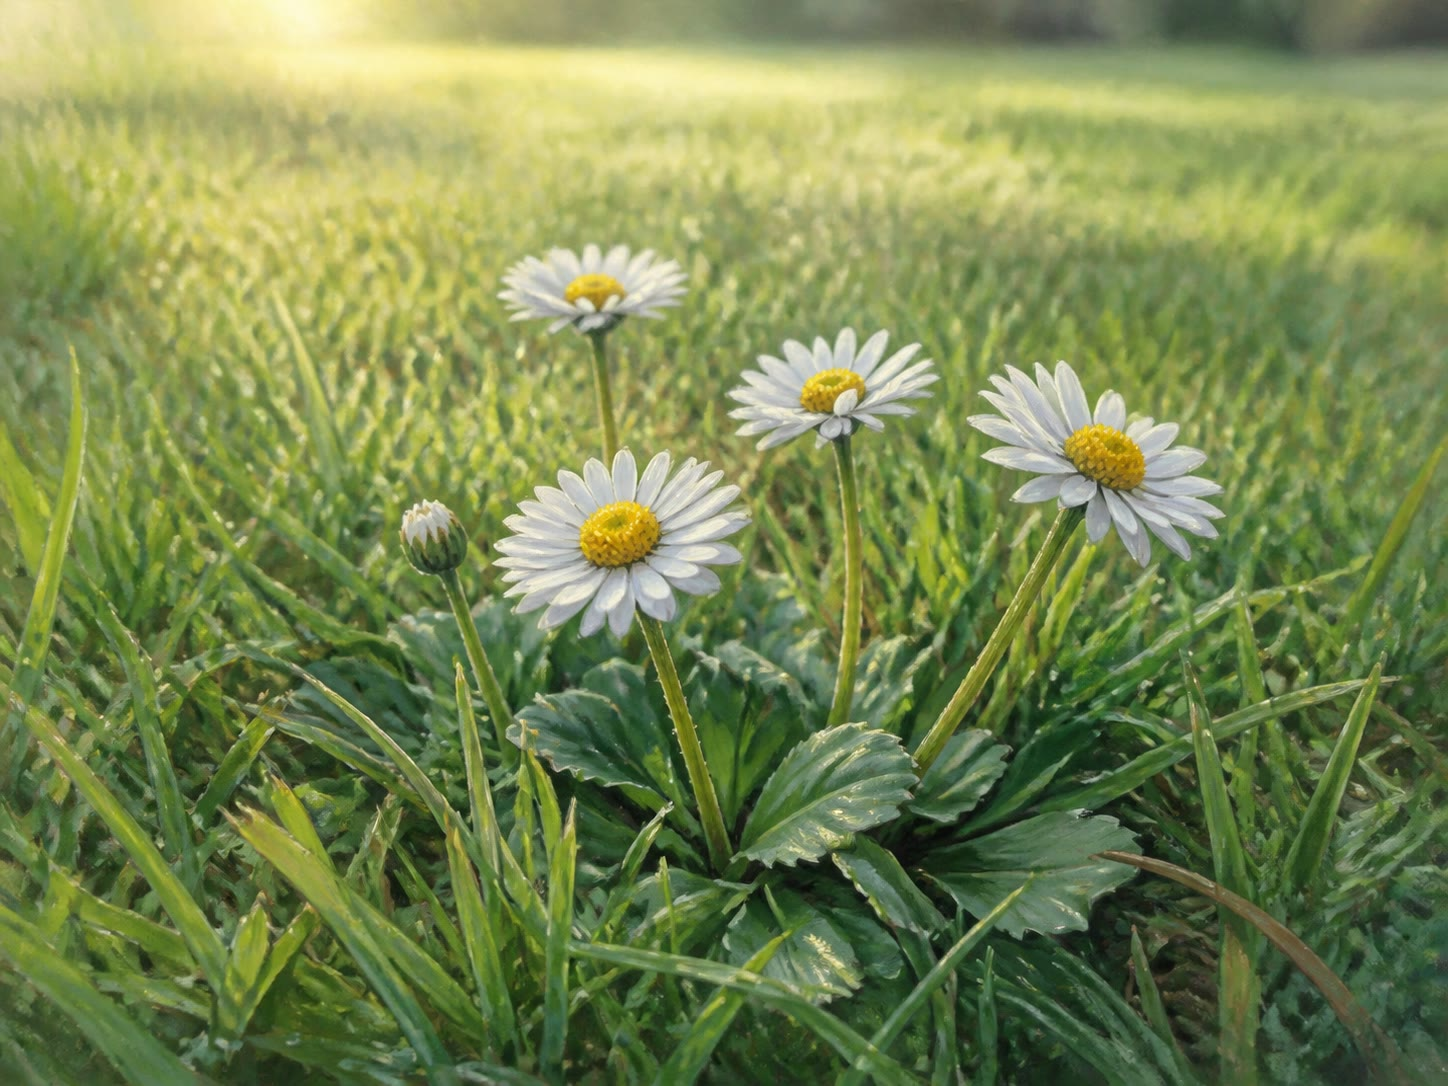
\includegraphics[width=0.58\linewidth]{images/book1/ai/g1-plants-daisy.jpg}

{\small 草坪上的雏菊：由种子长成，
靠光和水生长，安静地活着。}
\end{omfigure}

\begin{remark}[不动也是活的]\label{rem:g1:plants-around-us:still}
\omterm{def:g1:plants-around-us:plant}{植物}不会走路，但它们也并非完全静止。向日葵
白天会转向光源，跟着光走；窗台上的\omterm{def:g1:plants-around-us:plant}{植物}
会慢慢朝窗户的方向弯曲。\omterm{def:g1:plants-around-us:plant}{植物}靠
\emph{生长}来移动——对我们的眼睛来说太慢，
但连续观察一周，就能看出来。
\end{remark}

\section{植物的各部分}

\begin{definition}[植物的各部分]\label{def:g1:plants-around-us:parts}
一株开花\omterm{def:g1:plants-around-us:plant}{植物}有四个主要部分：
\begin{enumerate}
  \item \emph{根}\index{根}，藏在土壤里，
        负责固定植株并吸收水分；
  \item \emph{茎}\index{茎}，支撑植株直立，
        把水分输送到叶片；
  \item \emph{叶}\index{叶}，扁平且呈绿色，
        负责接收光照；
  \item \emph{花}\index{花}，将来会产生种子。
\end{enumerate}
\end{definition}

\begin{omfigure}
\begin{tikzpicture}
  \node[anchor=south west, inner sep=0] (img) at (0,0)
    {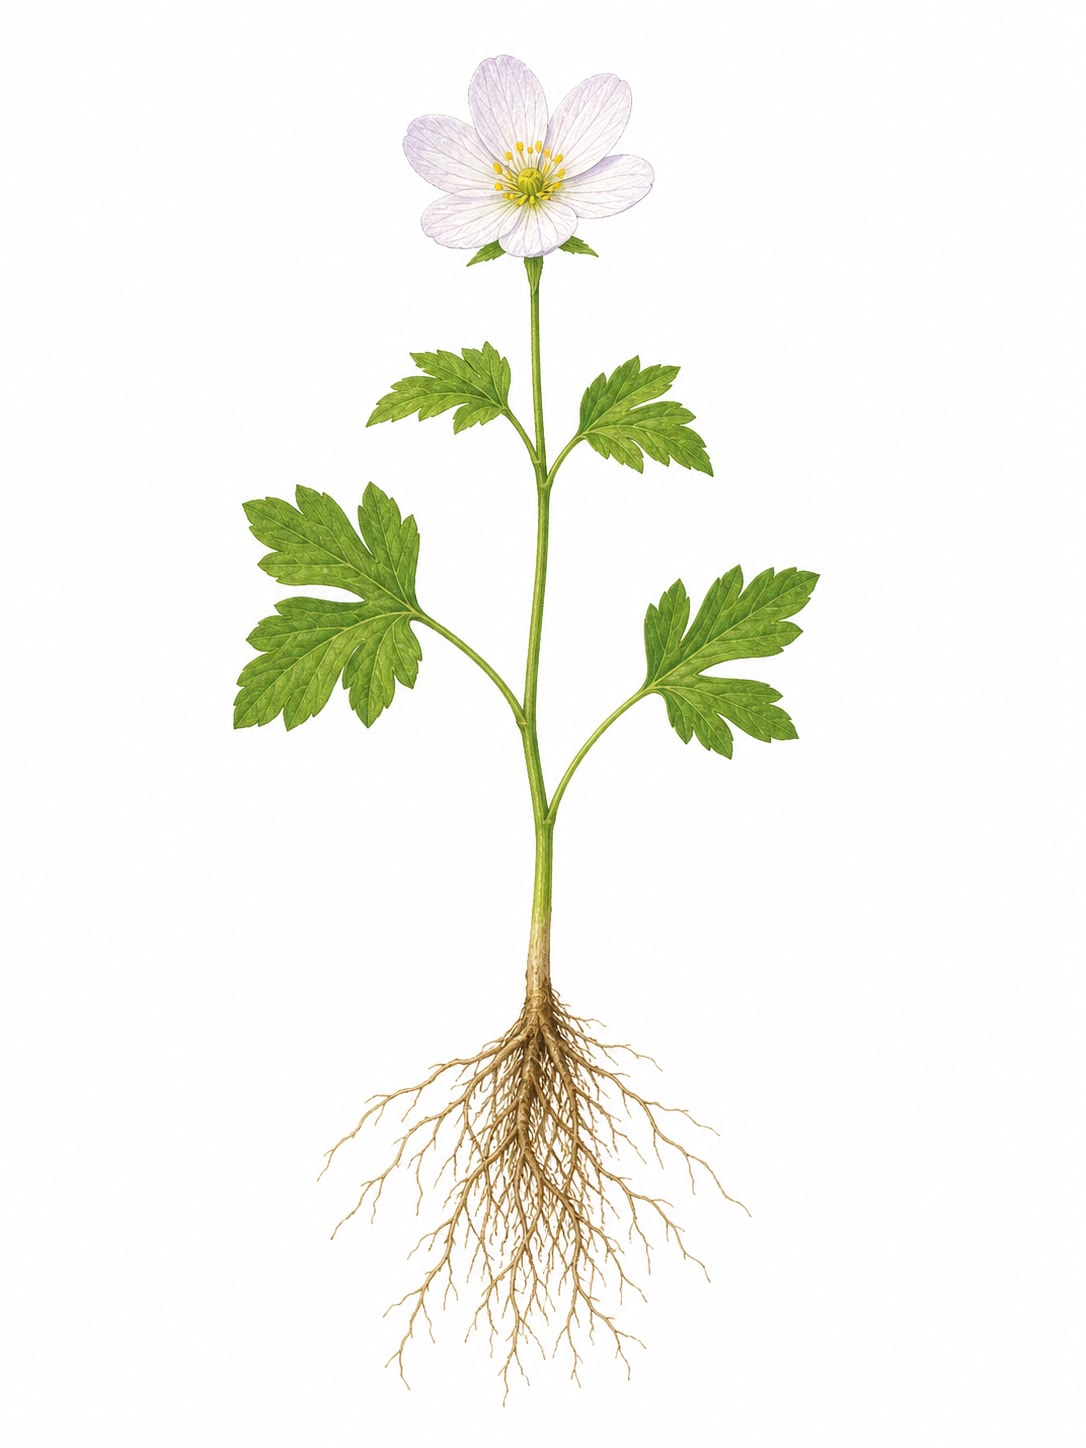
\includegraphics[width=0.5\linewidth]{images/book1/ai/fig-plant-uprooted.jpg}};
  \begin{scope}[x={(img.south east)}, y={(img.north west)},
      every node/.style={font=\small}]
    \draw[omDef, thick] (0.55,0.91) -- (0.74,0.93) node[right] {花};
    \draw[omDef, thick] (0.68,0.57) -- (0.84,0.62) node[right] {叶};
    \draw[omDef, thick] (0.51,0.33) -- (0.74,0.36) node[right] {茎};
    \draw[omDef, thick] (0.58,0.13) -- (0.78,0.16) node[right] {根};
  \end{scope}
\end{tikzpicture}

{\small 一株开花\omterm{def:g1:plants-around-us:plant}{植物}的四个部分，整株拔起展示：
根在地下，默默地在看不见的土壤里工作，
不为人见。}
\end{omfigure}

\begin{example}[拔一株杂草]\label{ex:g1:plants-around-us:weed}
轻轻地把一株杂草从松软湿润的泥土里拔出来，你会看到藏在下面的部分：
一撮浅色的根，有时比地面上整株绿色\omterm{def:g1:plants-around-us:plant}{植物}还长。
这样从下往上看，\omterm{def:g1:plants-around-us:plant}{植物}就清楚了：根、茎、叶，
如果运气好，还能看到一朵花。
\end{example}

\begin{definition}[树]\label{def:g1:plants-around-us:tree}
\emph{树}\index{树}是一种高大的\omterm{def:g1:plants-around-us:plant}{植物}，它的茎由木质构成。
树的木质茎称为\emph{树干}\index{树干}；
树干再分出\emph{分支}\index{分支}，
分支上长着叶。
\end{definition}

\begin{example}[栗树]\label{ex:g1:plants-around-us:tree}
院子里的栗树和雏菊的结构相同，
只是更大更硬：根在地下，树干代替了柔软的茎，
\omterm{def:g1:plants-around-us:tree}{分支}上有成千上万片\omterm{def:g1:plants-around-us:parts}{叶子}，春天还会开花。
雏菊只活一年，
而栗树可以活一百多年。
\end{example}

\section{植物需要什么}

\begin{proposition}[植物的需求]\label{prop:g1:plants-around-us:needs}
要活着并生长，\omterm{def:g1:plants-around-us:plant}{植物}需要\emph{水}、\emph{光}，以及
供根生长的地方，通常是\emph{土壤}\index{土壤}。
长期处于黑暗中或从不浇水的\omterm{def:g1:plants-around-us:plant}{植物}，会萎蔫并死去。
\end{proposition}
\admitted

\begin{example}[被遗忘的植物]\label{ex:g1:plants-around-us:wilt}
放假前忘了给教室里的\omterm{def:g1:plants-around-us:plant}{植物}浇水：它的\omterm{def:g1:plants-around-us:parts}{叶子}耷拉下来，
软软的，无精打采——\omterm{def:g1:plants-around-us:plant}{植物}萎蔫了。浇点水，
过几个小时\omterm{def:g1:plants-around-us:parts}{叶子}又会挺起来。缺的正是水。
\end{example}

\begin{method}[照顾植物]\label{met:g1:plants-around-us:care}
\begin{enumerate}
  \item 把花盆放在能晒到太阳的地方；
  \item 土壤感觉干了再浇水——不必每小时都浇，
        根也需要空气；
  \item 不要摘掉\omterm{def:g1:plants-around-us:parts}{叶子}：\omterm{def:g1:plants-around-us:parts}{叶子}是\omterm{def:g1:plants-around-us:plant}{植物}的
        接光器官；
  \item 要有耐心：\omterm{def:g1:plants-around-us:plant}{植物}几天才会有反应，不是几分钟。
\end{enumerate}
\end{method}

\begin{remark}[植物养活所有人]\label{rem:g1:plants-around-us:food}
\omterm{def:g1:plants-around-us:plant}{植物}对每一种\omterm{def:g1:animals-around-us:animal}{动物}都很重要。蜗牛吃沙拉，
乌鸫吃浆果，我们吃用小麦做的面包——小麦也是\omterm{def:g1:plants-around-us:plant}{植物}。
即使是不吃沙拉的猫，也吃那些吃过\omterm{def:g1:plants-around-us:plant}{植物}的\omterm{def:g1:animals-around-us:animal}{动物}。
没有\omterm{def:g1:plants-around-us:plant}{植物}，别的\omterm{def:g1:living-or-not:living}{生物}就没有东西可吃；后面
一章会讲这些食物链。
\end{remark}

\section{练习}

\begin{exercise}[$\star$]\label{exo:g1:plants-around-us:1}
说出开花\omterm{def:g1:plants-around-us:plant}{植物}的四个部分的名称，
从土壤下面直到顶端。
\end{exercise}

\begin{exercise}[$\star$]\label{exo:g1:plants-around-us:2}
哪一部分\omterm{def:g1:plants-around-us:plant}{植物}：（a）从土壤中吸水？（b）
接收光？（c）将会形成种子？（d）
使植株直立？
\end{exercise}

\begin{exercise}[$\star$]\label{exo:g1:plants-around-us:3}
雏菊从不走动。请列出生命的特征，
并说明它为什么仍然是\omterm{def:g1:living-or-not:living}{生物}。
\end{exercise}

\begin{exercise}[$\star$]\label{exo:g1:plants-around-us:4}
树的茎和承载树叶的部分，
各有什么专门的名称？
\end{exercise}

\begin{exercise}[$\star$]\label{exo:g1:plants-around-us:5}
根据
\cref{prop:g1:plants-around-us:needs}，说出\omterm{def:g1:plants-around-us:plant}{植物}生存所需的三样东西。
\end{exercise}

\begin{exercise}[$\star$]\label{exo:g1:plants-around-us:6}
教室里的\omterm{def:g1:plants-around-us:plant}{植物}\omterm{def:g1:plants-around-us:parts}{叶子}柔软、下垂。可能忘记了
什么？浇水之后会发生什么？
\end{exercise}

\begin{exercise}[$\star$]\label{exo:g1:plants-around-us:7}
雏菊和栗树在哪些方面相同？在
哪两个方面不同？
\end{exercise}

\begin{exercise}[$\star$]\label{exo:g1:plants-around-us:8}
试一试：把一株豆苗（或一盆水芹）放在窗边，
另一株放在黑暗的柜子里，两株都浇水，观察一周。
你预计会有什么不同？哪一种需要可以解释这种不同？
\end{exercise}

\begin{exercise}[$\star\star$]\label{exo:g1:plants-around-us:9}
利奥说：“\omterm{def:g1:plants-around-us:plant}{植物}并不是真的活着——它们
从来不做任何事。”请你举出\omterm{def:g1:plants-around-us:plant}{植物}慢慢但确实会做的两件事告诉他，
依据\cref{rem:g1:plants-around-us:still}和
\cref{ex:g1:plants-around-us:daisy}。
\end{exercise}

\begin{exercise}[$\star\star$]\label{exo:g1:plants-around-us:10}
胡萝卜是橙色的，生长在地下。看看\omterm{def:g1:plants-around-us:plant}{植物}各部分的
图，你认为我们吃的是胡萝卜\omterm{def:g1:plants-around-us:plant}{植物}的哪一部分？
“长在地下”这一提示说明了什么？
\end{exercise}
